\documentclass[11pt,a4j,ascmac]{jarticle}
\usepackage{epsf}
\usepackage[dvips]{graphicx}

\setlength{\textheight}{25cm}
\setlength{\textwidth}{16cm}
\setlength{\topmargin}{-2.5cm}
\setlength{\oddsidemargin}{0mm}
\setlength{\parindent}{0pt}
\setlength{\parskip}{3mm}


\title{第8月 進捗確認会報告資料\\
Tensorflow動作環境について}

\author{ER17076  安井 理}
\date{2020年 9月 9日}
\begin{document}
\maketitle


\section{はじめに}

\  今月はTensorflolw-gpuの動作しない問題についてと,今後のやる事を明確にして方針を明らかにすることを目的とし大学側のパソコンの環境設定,Tensorflolwの調査を主に研究をしてきた.



\section{進捗報告}



\subsection{調査内容}

\begin{description}
  \item ・6Dとは
 \item ・Tensorflow-gpuの環境調査
 \item ・今後の方針について
\end{description}



\subsection{6次元推定の概要}
\  

\subsection{3Dについて}

\  まず,3Dの理解として,3DoF(3D推定)図\ref{fig:3D}に示すように,pitch・yaw・rollのXYZ軸周りの3つの回転に対する推定.
\\ 

      \begin{figure}[htpp]
      \centering
      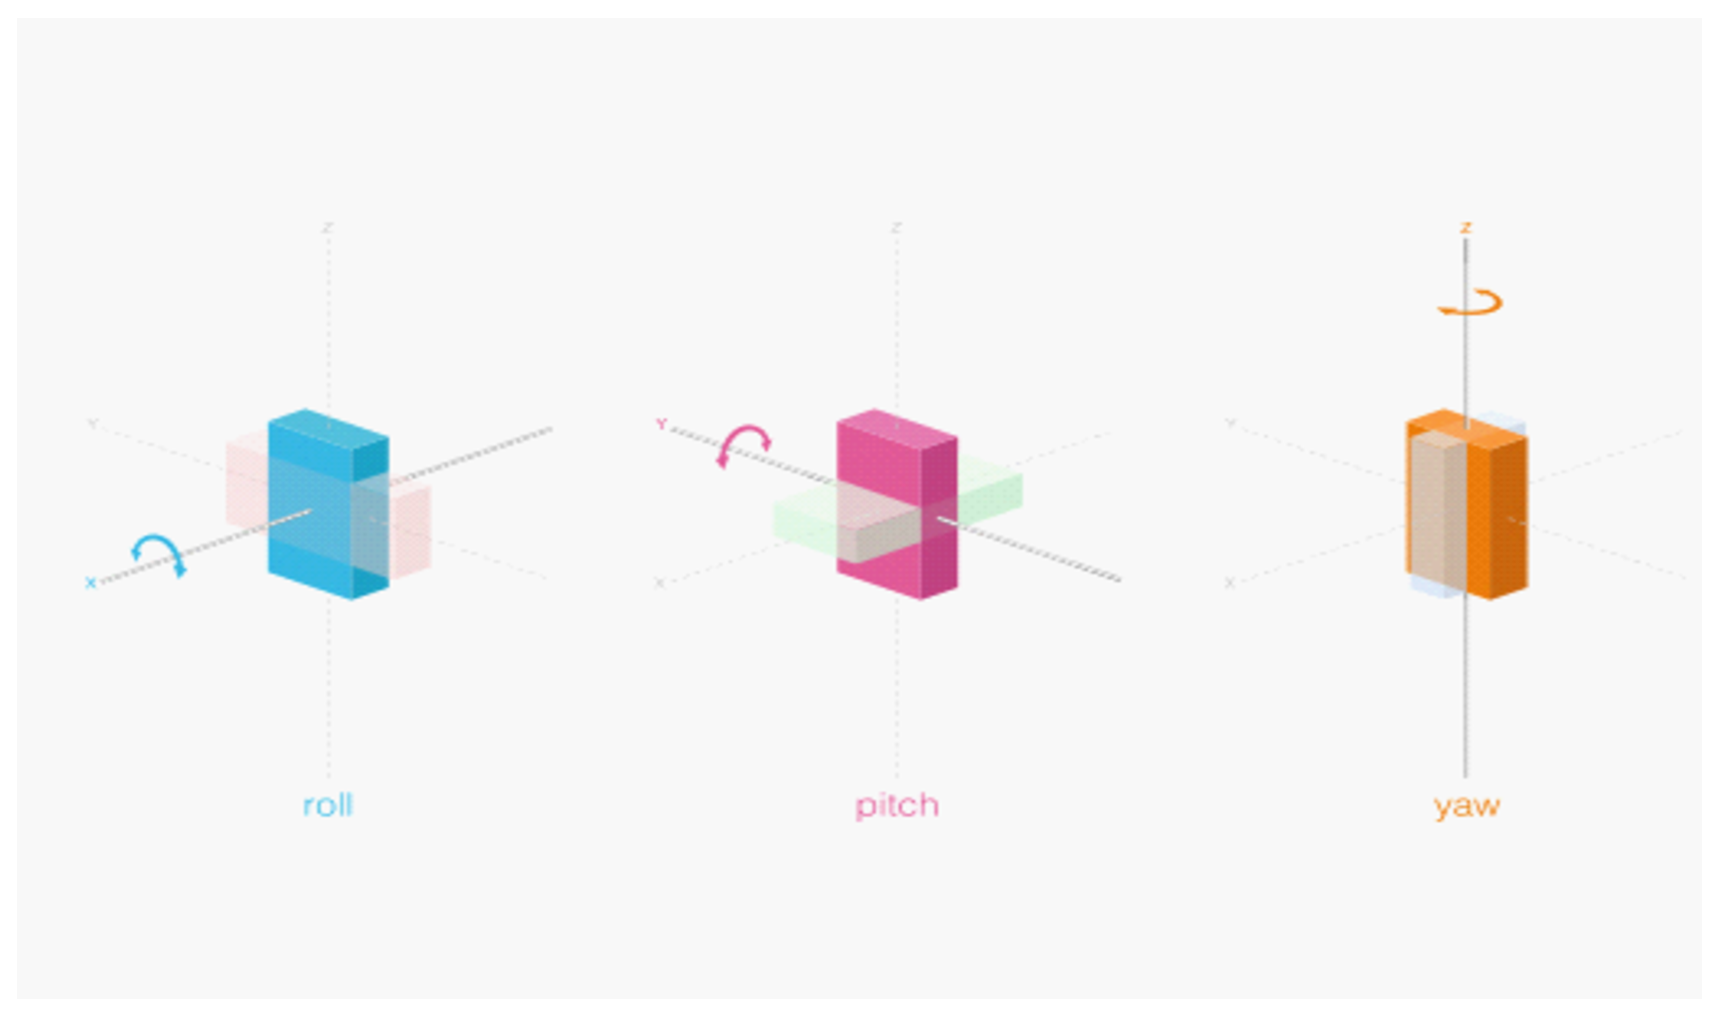
\includegraphics[width=100mm]{3D.eps}
      \vspace*{20mm}
      \caption{3D推定.}
      \label{fig:3D}
      \end{figure}

\subsection{6Dについて}
\  6Dは,前後・左右・上下 のXYZ軸周りの3方向の動きに対する推定で物体の移動推定というより,図\ref{fig:6D}に示すように,物体を捉えるカメラ視点の移動推定を指すものである.イメージとして物体の回転(3D)+カメラ位置(3D)の推定が6D推定である.


      \begin{figure}[htpp]
      \centering
      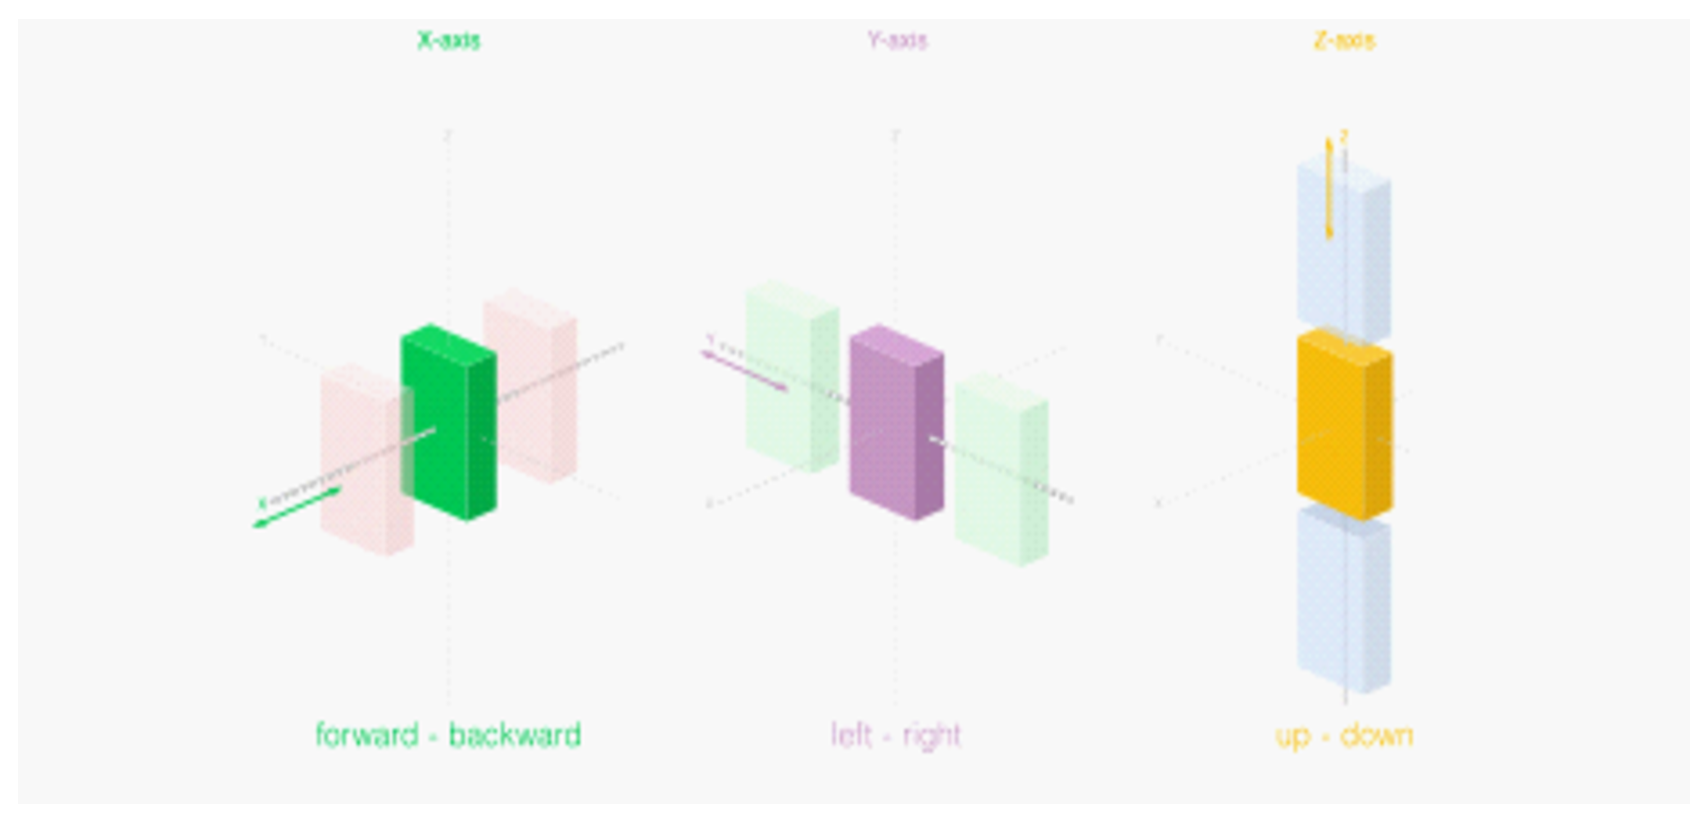
\includegraphics[width=100mm]{6D.eps}
      \vspace*{20mm}
      \caption{6D推定.}
      \label{fig:6D}
      \end{figure}






\subsection{Tensorflow-gpu動作環境}


\subsubsection{Tensorflowについて}
\  機械学習の分野で使用するためのOSS(オープンソフトウェアライブラリ)であり,開発元がGoogle Brainチーム.対応OS: Linux, macOS, Windows, Android, iOS... 対応言語:C言語,C++,Python,Java,Goなどと機械学習の分野で幅広く使用されるものである.\\ 

\  主に以下の特徴が挙げられる

\begin{description}
  \item ・データの読み込み、前処理、計算、状態、出力などを多次元的に処理する
 \item ・分散処理が可能なためビッグデータ(大量のデータ)も扱える
\end{description}


\subsubsection {OSS}
\  ソースコードの学習や変更・配布することが認められているライブラリ


\subsubsection{現状確認}
\  Tensorflow(CPU)が動作することは確認済み(学習可能)のため,Tensorflow-GPUがプログラムの問題で動作しない or PCの問題で動作していないかを調査する.PCがTensorflow-GPUを認識しているかをサイト[https://thr3a.hatenablog.com/entry/20180113/1515820265]を参考に調査をした,結果として,PCが認識していないことが分かった.\\

\  調査結果としてPCがGPUを認識していなかったため、条件を変えながら行った.調査結果を図\ref{fig:survey}に示す.

      \begin{figure}[htpp]
      \centering
      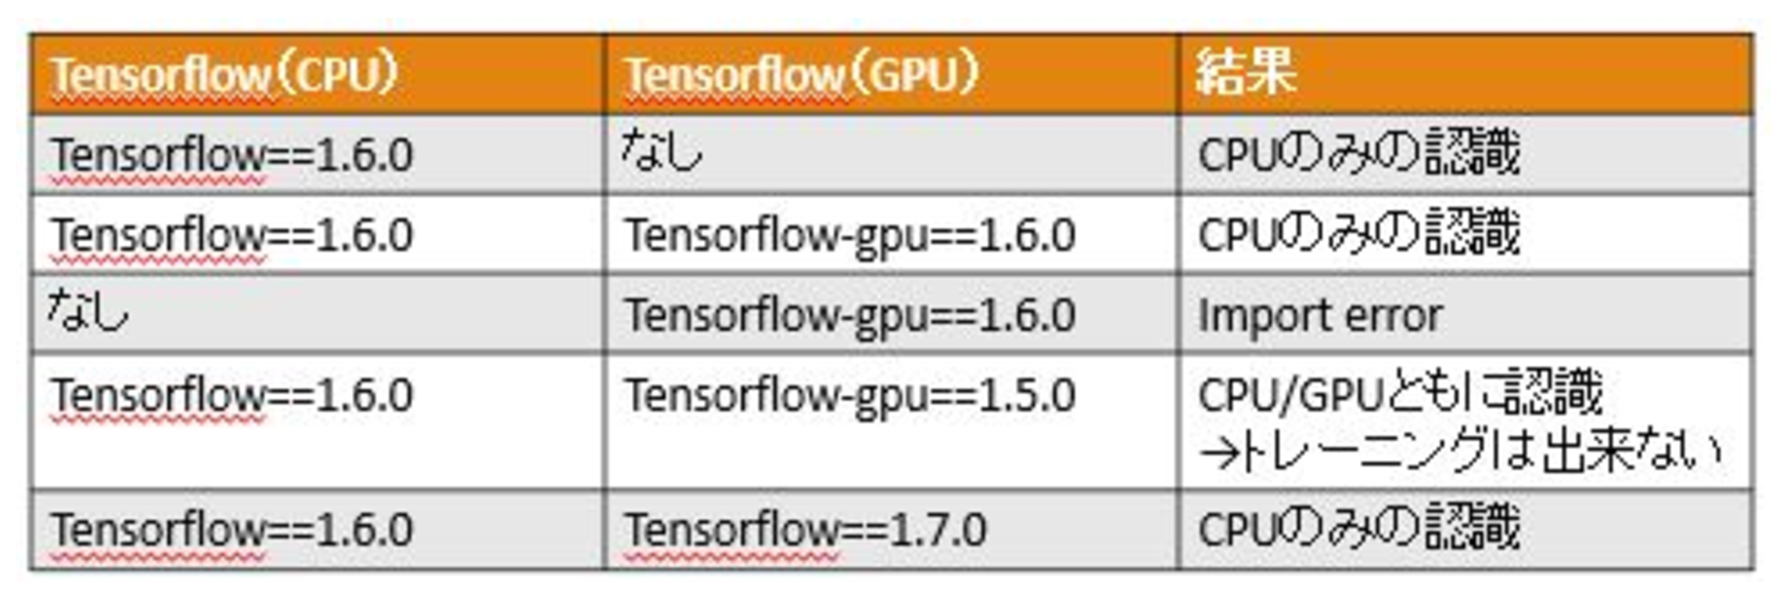
\includegraphics[width=100mm]{調査結果.eps}
      \vspace*{20mm}
      \caption{調査結果.}
      \label{fig:survey}
      \end{figure}


\  Tensorflowの色々なバージョンを試したがGPUは認識されなかった,Tensorflow-GPUをダウングレードした時のみ認識したが,git-hubのコードに非対応のため動作できなかった.今回の問題は,Tensorflowそのものでなく他の環境のバージョンとの問題であると考えた



\subsubsection{CUDA・cuDNN環境}

\  CUDAとcuDNNのバージョンを確認し,CUDA9・cuDNN7となっており推奨のバージョンであることを確認した.念のためもう一度インストールしなおす(cuDNNは7.4.1ではTensorflowが動作しない)CUDA9.0・cuDNN7.1.4を入れ直し再起動.

\  再起動後にログインループしてしまい,ubuntu14.04・ctrl+Alt+F1(コンソール)も操作不可能,グラフィックボードを抜いた状態だと操作可能になった.その為,labinfo・PC型番を参考にNVIDIAドライバー(nvidia-430)を再インストール・再起動を行った,するとグラボがある状態での操作が可能になった.

\  しかし,再度CUDA・cuDNNをインストールし再起動するとログインループの状態になり,NVIDIAのほかのバージョンを試しても同じ現象が起こった.nvidia-smiで確認したところlibrary version mismatchと表示されていたので,バージョンはあっているが何かが邪魔をしている可能性があると考えられる.





\subsection{今後の方針}
\  ubuntuを入れ直して初めからやり直す,問題として鈴木さんの研究(Faster-RCNN)を動かす環境もやり直す必要が出てくるので大切なファイルのバックアップ・環境の記録を残す必要がある.再インストール後に引き続きAAEの実装を行う.Tensorflow-gpuが認識するように環境を構築する


\subsection{終わりに}
\  今月は研究内容を進められなく,PCの環境設定に時間を多く取られてしまい自分の思うように進められていないので環境設定が終わり次第に自分のやりたいことができるように,環境作りをしながら目標を明確にやっていくことを考えながらまとめていきたいと思う.PC環境の知識が全くないのでこういう機会に少しでも理解して,基礎知識の幅を増やして行くことも大切だと思った.

\footnotesize



\normalsize

\end{document}
